\documentclass{scrartcl}

\usepackage[hidelinks]{hyperref}
\usepackage[none]{hyphenat}
\usepackage[utf8]{inputenc}
\usepackage{csquotes}
\usepackage{blindtext}
\usepackage{enumitem}
\usepackage{xcolor}
\usepackage{graphicx}
\graphicspath{ {images/} }

\title{COMP350-Research Journal}
\subtitle{Optimisation of Games}

\author{1506530}

\begin{document}
	
	
	\maketitle
\section{Introduction}
	In the games industry there are many types of optimisation methods and tools, one such tool is the unreal profiling tool \cite{UEPer}, which includes a detailed breakdown of everything that runs in the game loop. Amongst the unreal tools are also a Graphics Processing Unit (GPU) profiler, and a asset statistics sheet, there are more ways to get an overview of what is happening in the engine which shall be covered in this journal. The main point of this journal is to provide a foundation for optimizing a game within the unreal engine providing both about the tool and how to use it.
	
\section{Optimisation in Unreal}
Optimisation making the most out of the available resources. In games this is usually attributed to gaining the most Frames per Second (FPS) out of your system \cite{UEYouTube}, and in Unreal this can be done in several ways, a list of which can be found at the Unreal Documentation. In this journal an overview of some of the tool will be presented with examples on how to use them.

The first step is to find the bottleneck and see whether its in the CPU or GPU or in the Game (Your Code). Unreal provides a command \textquote{stat.unit} which displays statistics similar to image 1. In this example the Frame and GPU are very close in value, this means that the bottleneck is the GPU. If it were the CPU then the Draw would be close, and if its your code then the Game will be. The best way to discover which this is is by launching a release build of the game and typing the command, then noting the values. Once you have discovered the bottleneck then the next move is to use the appropriate profiler to fix the issue.

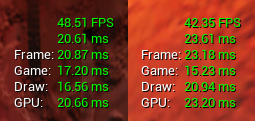
\includegraphics{Image1}

\section{CPU Profiling}
Being CPU bound means that there are too many draw calls, this is an issue that artists can help overcome by combining multiple assets into one larger asset. Having multiple instances of the same material can increase the draw time and can be resolved by using a material instance. The CPU render thread also handles processing objects, GPU commands and graphics drivers \cite{UECPU}.

\subsection{Code Optimisation}
Another way you can be CPU bound is in te game thread in this instance using the session frontend profiler will give you an idea of where the CPU is begin slowed. To begin finding this a use of the command \textquote{stat startfile} when running the game and then \textquote{stat stopfile} when the game has been run for a period of time. This action will record and save data from the game which can then be opened in the session frontend window and inspected. This is related to the games code, which in itself can be a maze to find the issue, one common pitfall is the \textquote{FTickFunctionTask} which is the tick for every actor and component with one. Reducing the number of actors that tick or introducing a delay to tick triggers can help reduce this issue \cite{BlogUnreal}.

\section{GPU Profiling}
The GPU profiler shows the user how much each rendered object uses during runtime, this can allow thw user to quickly identify any cost for the various passes. There are two types of GPU profilers in Unreal, one text version and one with a mouse based UI. Both have their merits and both have limitations
\newline
Mouse Based UI:
\begin{description}[font=$\bullet$~\normalfont\scshape\color{red!50!black}]
\item You can see greater level of information for the high level costs, for example you can see exactly what is causing the PrePass to be of a high cost by clikcing on it.
\item Unfortunately this does not give a real time running cost view of the game, the information is given from data taken from the frame it is called on.
\item It can not be used during the release version of the game.
\item Some drivers can optimise shaders before the GPU profiler uses the data so it can produce false numbers.
\end{description}

Text:
\begin{description}[font=$\bullet$~\normalfont\scshape\color{red!50!black}]
\item Unlike the mouse based UI you can not see much information passed the high level names of the pass.
\item The text can give a real time running cost of the game allowing for greater accuracy and finding trouble areas.
\item The text can be used during the release build.
\end{description}

To access the GPU text profiler just type the command \textquote{stat.gpu} and a wall of text will appear ingame as seen in image 2. Using the same \textquote{stat start/stopfile} command you can load the ingame GPU information into the frontend tool for reviewing \cite{UEGPU}.

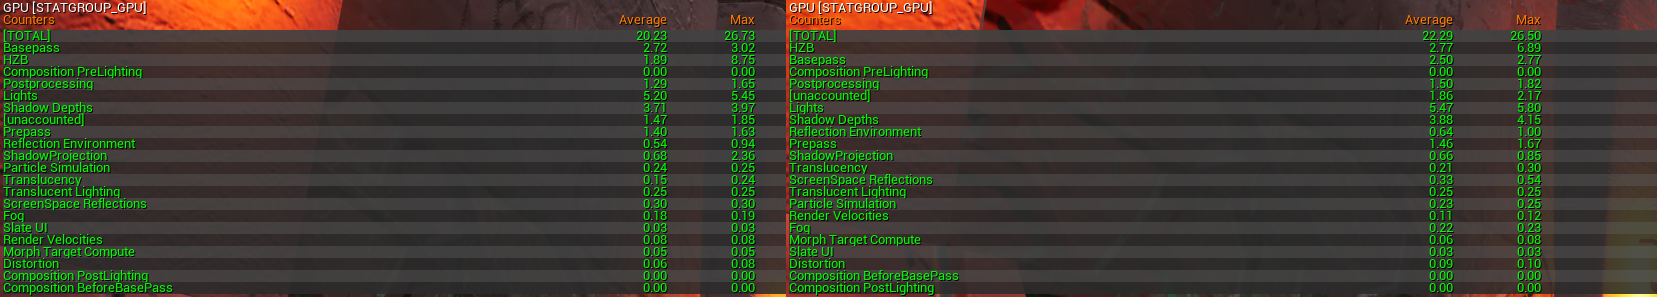
\includegraphics[width=\textwidth]{Image2}

\section{Content Optimisation}
Simply put content optimisation is the process of optimising the objects that are rendered ingame, including the meshes, animations and lighting. Though lighting can be dealt with using the GPU profiler there are other ways to identify the issue,	 though in this instance the meshes are the focus. Unreal provides a Mesh statistics profiler that is a spreadsheet of data that contains various pieces of information that can help to identify any suspect meshes \cite{Content}. As can be seen in image 4, there are several meshes referencing a 4K texture files when they do not need to, this can be easily rectified by selecting the asset and editing the max resolution.

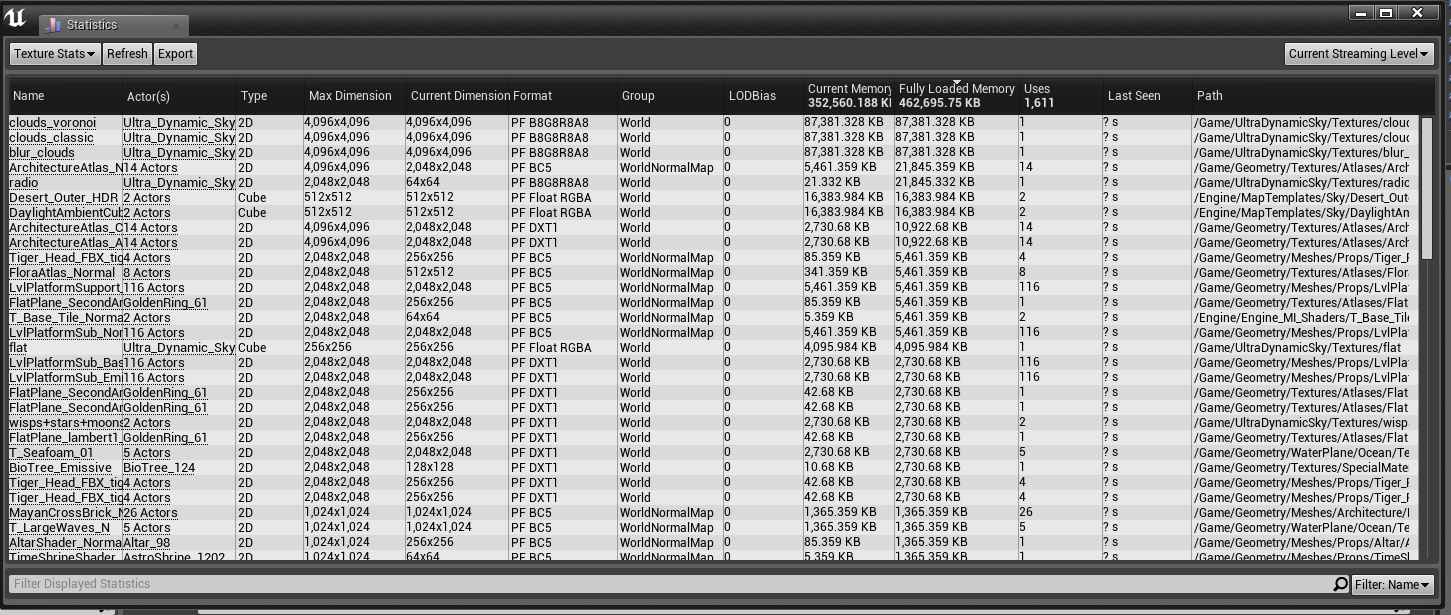
\includegraphics[width=\textwidth]{Image3}

\section{Final Remarks}
There are many tools in Unreal that can help developers identify and rectify issues within their game to ensure it runs at maximum efficiency. Though there are many more than those described in this journal, the ones mentioned here cover the basics. When planning on optimizing work it is always best to plan ahead and try to optimise during development and not to optimise at the end, as this can reveal larger issues within your program that may require a larger amount of time and effort to fix than is available \cite{UEPerformance}.
	
	
	
	\bibliographystyle{IEEEtran}
	\bibliography{COMP250-Journal}
	
\end{document}